%% LyX 2.2.2 created this file.  For more info, see http://www.lyx.org/.
%% Do not edit unless you really know what you are doing.
\documentclass[english]{beamer}
\usepackage{mathptmx}
\usepackage[latin9]{inputenc}
\usepackage{amsmath}
\usepackage{amssymb}
\usepackage{graphicx}
\usepackage[european]{circuitikz}
\ctikzset{tripoles/mos style/arrows}

\makeatletter

%%%%%%%%%%%%%%%%%%%%%%%%%%%%%% LyX specific LaTeX commands.
%% Because html converters don't know tabularnewline
\providecommand{\tabularnewline}{\\}

%%%%%%%%%%%%%%%%%%%%%%%%%%%%%% Textclass specific LaTeX commands.
 % this default might be overridden by plain title style
 \newcommand\makebeamertitle{\frame{\maketitle}}%
 % (ERT) argument for the TOC
 \AtBeginDocument{%
   \let\origtableofcontents=\tableofcontents
   \def\tableofcontents{\@ifnextchar[{\origtableofcontents}{\gobbletableofcontents}}
   \def\gobbletableofcontents#1{\origtableofcontents}
 }

%%%%%%%%%%%%%%%%%%%%%%%%%%%%%% User specified LaTeX commands.
\usetheme{Warsaw}
% or ...

\setbeamercovered{transparent}
% or whatever (possibly just delete it)

\makeatother

\usepackage{babel}
\begin{document}

\title[Designing a SCaM]{Analog Design for a Single-Chip atto Mote (SCaM) Microcontroller
}

\author[Kevavi]{Kevin Chen, Avi Pandey, Kevin Zheng}

\institute{University of California, Berkeley}

\date{Presentation 2}

\makebeamertitle

%\pgfdeclareimage[height=0.5cm]{institution-logo}{logo.png}
%\logo{\pgfuseimage{institution-logo}}

\AtBeginSubsection[]{%
  \frame<beamer>{ 
    \frametitle{Outline}   
    \tableofcontents[currentsection,currentsubsection] 
  }
}

%\beamerdefaultoverlayspecification{<+->}
\begin{frame}{Outline}

\tableofcontents{}
\end{frame}

\section{Preliminary Results of Integration}

\subsection{Integration}
\begin{frame}{Semi-Ideal SCaM Overview}
\begin{itemize}
\item SCaM is alive!
\item Atleast with ideal op-amps
\item Slowly adding completed and real op-amp blocks into the integration one by one in order to isolate problems caused by individual blocks \begin{itemize}
\item Strong Arm Latch
\item V$_{ref}$ regulator
\item PGA*
\item Digital regulator*
\end{itemize}
\end{itemize}
\end{frame}
%
\subsection{Error Results}

\begin{frame}{Ideal Full System LSB Error I}
\begin{itemize}
\item Selected analog input of 100 mV DC
\item PGA set to gain of 8
\item Tabulated worst case error in number of LSB
\end{itemize}
\begin{center}
Temperature ($^\circ$C) \& Battery Voltage (V) \\
\begin{tabular}{|c|c|c|c|}
\hline
& 1.6 V & 2.4 V & 3.2 V \tabularnewline \hline
70 $^\circ$C & 0 & 0 & 0\tabularnewline 
\hline
25 $^\circ$C & $V_{ref}$ broken & 0 & 0\tabularnewline
\hline
0 $^\circ$C & 0 & $V_{ref}$ broken & 0 \tabularnewline 
\hline 
\end{tabular}
\end{center}
($V_{ref}$ is completely not working in some scenarios, and yielding an ADC output of all zeroes) \\
\end{frame}
%

\begin{frame}{Ideal Full System LSB Error II}
\begin{itemize}
\item Selected temperature sensor input
\item PGA set to gain of 1
\item Tabulated worst case error in number of LSB, below
\end{itemize}
\begin{center}
Temperature ($^\circ$C) \& Battery Voltage (V) \\
\begin{tabular}{|c|c|c|c|}
\hline
& 1.6 V & 2.4 V & 3.2 V \tabularnewline \hline
70 $^\circ$C & 996mV & 843.8mV & 843.8mV\tabularnewline 
\hline
25 $^\circ$C & $V_{ref}$ broken & 820.3mV & 820.3mV\tabularnewline
\hline
0 $^\circ$C & 976.53mV & $V_{ref}$ broken & 804.6mV \tabularnewline 
\hline 
\end{tabular}
\end{center}
\end{frame}
%

\begin{frame}{PGA LSB Error}
\begin{itemize}
\item Input of 200 mV
\item PGA set to gain of 1
\item Ideal supply voltage of 1.2V
\item Tabulated worst case error in number of LSB, below
\end{itemize}
\begin{center}
Temperature ($^\circ$C) \\
\begin{tabular}{|c|c|}
\hline
70 $^\circ$C & 0 \tabularnewline 
\hline
25 $^\circ$C & 21 \tabularnewline
\hline
0 $^\circ$C & 15 \tabularnewline 
\hline 
\end{tabular}
\end{center}
With the PGA, all other gain settings were within 1 LSB of error, and only unity gain was giving problems
\end{frame}
%

\section{Progress and Design Decisions}

\subsection{Ideal Blocks and Topologies}
\begin{frame}{BGT \& REG}
\begin{block}{Basic Performance}
\begin{itemize}
\item IS ALIVE WITH 1.2135-ISH VOLTS FOR BG/REGS, 1 VOLT FOR VREF
\end{itemize}
\end{block}
%
\begin{block}{Notable Design Decisions}
\begin{itemize}
\item Used PSR band gap reference - Li, Yao, Guo 2009
\item V$_{ref}$ LDO replaced with unity gain buffer
\end{itemize}
\end{block}
\end{frame}
%
\begin{frame}{MUX \& PGA}
\begin{block}{Basic Performance}
\begin{itemize}
\item MUX settles within 100 ns
\item PGA's amplified results stay within 0.4\% error for the 5 $\mu$s window of the "amplify" phase
\end{itemize}
\end{block}
%
\begin{block}{Notable Design Decisions}
\begin{itemize}
\item Mostly minimum size transistors for switching
\item Used hvt devices for less leakage in transmission gates
\item Used nmos2v in parallel with $C_f$ across the op-amp
\item Used fairly large capacitors to prevent voltage drooping and charge injection
\end{itemize}
\end{block}
\end{frame}
%
\begin{frame}{ADC}
\begin{block}{Basic Performance}
\begin{itemize}
\item Accurate with an ideal supply
\item Uses a 10MHz digital clock
\end{itemize}
\end{block}
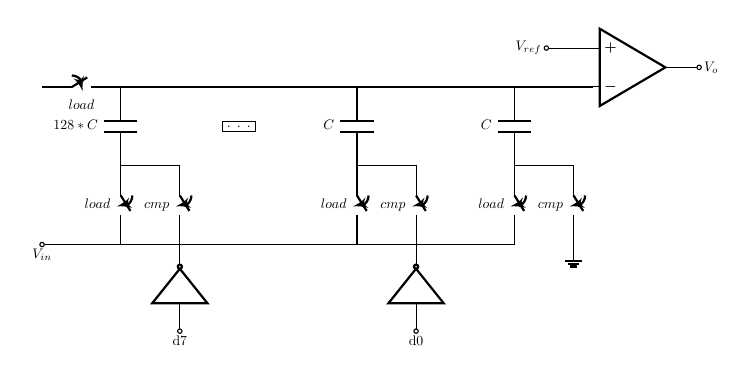
\begin{tikzpicture}[scale = 0.5, transform shape]
    \draw
    (0,4) 
    to[spst, l_=$load$] ++(2,0)
    to[short] ++(12,0)
    
    (2,4)
    to[C, l_=$128*C$] ++(0,-2)
    to[spst, l_=$load$] ++(0,-2)
    to[short, -o] ++(-2,0)
    node[anchor=north]{$V_{in}$}
    
    (2,2)
    to[short] ++(1.5,0)
    to[spst, l_=$cmp$] ++(0,-2)
    
    (3.5,-1)
    node[american not port, rotate = 90] (inv1) {}
    (inv1.out) -- (3.5,0)
    (inv1.in) to[short, -o] ++(0,-0.5)
    node[anchor=north]{d7}
    
    (8,4)
    to[C, l_=$C$] ++(0,-2)
    to[spst, l_=$load$] ++(0,-2)
    to[short] (0,0)
    
    (8,2)
    to[short] ++(1.5,0)
    to[spst, l_=$cmp$] ++(0,-2)
    
    (9.5,-1)
    node[american not port, rotate = 90] (inv1) {}
    (inv1.out) -- (9.5,0)
    (inv1.in) to[short, -o] ++(0,-0.5)
    node[anchor=north]{d0}

    
    (12,4)
    to[C, l_=$C$] ++(0,-2)
    to[spst, l_=$load$] ++(0,-2)
    to[short] (0,0)
    
    (12,2)
    to[short] ++(1.5,0)
    to[spst, l_=$cmp$] ++(0,-2)
    node[ground]{}

    (15,4.5) node[op amp, yscale=-1](comp){} 
    (comp.+) to[short, -o] ++(-1,0)
    node[anchor=east]{$V_{ref}$}
    
    (comp.out) to[short,-o] ++(0.5,0)
    node[anchor=west]{$V_o$}

    node[draw] at (5,3) {. . .}
    ;
\end{tikzpicture}

\end{frame}
%
\begin{frame}{ADC - Leakage}
\begin{block}{Charge Leakage}
\begin{itemize}
\item d7 and d6 overlap (thanks Brad), causes unexpectadly high voltages
\item High leakage current causes more than an LSB of loss.
\end{itemize}
INCLUDE GRAPHIC HERE
\end{block}
\end{frame}

\begin{frame}{ADC- Charge Pump}
\begin{block}{Charge Pump Topolgy}
\begin{itemize}
\item Using a charge pump to reduce the $V_{GS}$ of the Load PMOS
\item Restricts leakage to less than an LSB
\end{itemize}
\end{block}
\begin{circuitikz}[scale=0.5, transform shape]
    \draw
    (0,0) node[pmos, rotate=90](pmos1){}
    (pmos1.S) to[short,-o] ++(-1,0)
    node[anchor=north]{$V_{ref}$}
    
    (-1,1.5) node[nmos,rotate=90](nmos1){}
    (pmos1.S) to[short] ++(-1,0)
    |- (nmos1.D)
    (nmos1.G) -| (-1.8,0.5)
    (nmos1.S) to[short] ++(0.28,0)
    to[short] ++(0,-1.9)  
    
    (1,-1.5) node[pmos, rotate=90](pmos2){}
    (pmos2.S) -| (pmos1.G)
    (pmos2.D) to[short] (3,-1.5)
    |- (nmos1.S)    
    
    (0,-3.5) node[nmos, xscale=-1](nmos2){}
    (nmos2.D) -- (pmos1.G)
    (nmos2.G) -| (pmos2.G)
    
    (1, -5) node[american not port, rotate=90](inv1) {}
    (inv1.out) |- (nmos2.G)
    (inv1.in) -| (nmos2.S)
    (inv1.in) -| (3,-3.5)
    (3,-3.5) to[C, l_=$C_{hold}$] ++(0,2)
    
    (inv1.in) to[short,-o] ++(0,-0.5)
    node[anchor=west]{load\_b}

    (pmos1.D) to[short] ++(4,0)
    ;
\end{circuitikz}

\end{frame}

\begin{frame}{ADC - Charge Pump cont.}
Insert diagrams here
\end{frame}

\subsection{Clocking Details}
\begin{frame}{Clocking with the PGA and ADC}
\begin{itemize}
\item Synchronized PGA "$\phi_1$", the "sample" phase, with the ADC's "compare" phase, and the PGA's "$\phi_2$, or "amplify", with the ADC's "load" phase
\item $\phi_1$ and $\phi_2$ are 5 $\mu$s each, with rise and fall times of 10 ns, and thus the clock period of 10 $\mu$s satisfies the 100ksamples/s required by spec
\item ADC clock (10MHz) is equal to digital clock
\item We deliberately delayed the digital clock by 10ns so that it would not interfere with rise/fall times of $\phi_1$ and $\phi_2$, as it was previously causing the ADC to raise the MSB 100\% of the time
\end{itemize}
\end{frame}
%
\subsection{Real Op-amps (In Progress)}
\begin{frame}{BGT \& REG}
\begin{itemize}
\item Voltage Reference (finished):
\begin{itemize}
\item In unity gain configuration
\item Can handle anywhere from 8fF to 2pF+ loads
\end{itemize}
\item Digital Regulator ("finished"):
\begin{itemize}
\item Current version either oscillates very frequently or has a large variation from the intended band gap voltage
\item Planning to make a "slow" amplifier to avoid pulse-y behavior
\end{itemize}
\item Analog Regulator:
\begin{itemize}
\item Make "slow" to complement digital regulator
\item Still need to think about a way to provide as little variation as possible
\end{itemize}
\item Band Gap Reference
\end{itemize}
\end{frame}
%
\begin{frame}{PGA}
\begin{itemize}
\item Two Stage PMOS Input Cascode:
\begin{itemize}
\item Having problems with leakage while holding across a clock cycle
\item Can drive to within 3mV of ground using second stage NMOS input
\end{itemize}
\item Topology:
\begin{itemize}
\item Extra grounding switch added to $\phi_1$ discharge caps when V- cannot be driven to 0V fast enough
\end{itemize}
\end{itemize}
\end{frame}

\begin{frame}{ADC}
\begin{itemize}
\item Strong Arm Latch - Scott, Boser, Pister 2003:
\begin{itemize}
\item Used $\overline{RST}$ = CLK
\end{itemize}
\end{itemize}
\end{frame}
%
\section{Moving forward}
\subsection{Priorities}
\begin{frame} {Remarks on Potential Problems}
\begin{itemize}
\item Ensure band gap reference and voltage regulators work!
\begin{itemize}
\item Buggy band gap and unstable regulated voltages caused LOTS of trouble even during ideal integration
\end{itemize}
\item PGA needs to be able to hold its amplified voltage for as long as possible, without drooping too far away from its initial position
\item Temperature actually hasn't seemed to be too big of a problem so far, though they gave the biggest problems during labs 4 and 5
\end{itemize}
\end{frame}

\subsection{Responsibilities}
\begin{frame}{Recap of Milestones}
\begin{itemize}
\item Blocks complete and implemented with ideal amplifiers (4/20)
\item System-level testbenches complete; first integration (4/21)
\item Ideal amplifiers replaced with real amplifiers (4/25)
\item Sanity check and verification (4/26)
\item Extras, final integration and submission (4/28)
\end{itemize}
\end{frame}
%


\end{document}
